\chapter{QUIC协议评估}
本章的主要内容是将QUIC协议与TCP协议进行了传输任务的吞吐量进行对比,主要分为了在单机进行的仿真测试和真实网络流量情况下两个主机之间的传输测试。其中单机的仿真测试使用的拓扑包括了简单的一对一的拓扑,以及具有瓶颈电路的哑铃状拓扑。而在两个主机之间的传输测试包括了在一个机器上的两个进程分别运行的客户端和服务端之间的传输以及两个不同机器上运行的客户端和服务端之间的传输。

\section{仿真方案设计}
仿真的方案设计如下:由客户端在一段时间内,通过相应的协议(QUIC或者TCP)向服务端发送随机字符串,而服务端会输出已经成功收到的字节数,通过改变仿真的网络状况参数以及网络拓扑,还有客户端发送数据的流量模式(比如在泊松流的情况下)来对QUIC和TCP协议进行详尽的评估测试。
\subsection{网络参数设置}
网络参数主要与链路有关,主要参数有网络传输延迟(Delay)、链路带宽(BandWidth)、丢包率(Loss);除此以外,在哑铃状拓扑中,其瓶颈电路的带宽(MidBw)也是一个重要的参数。在整个仿真过程中,这些参数会被设置为xxx(用什么格式比较好)

\subsection{网络拓扑}
使用的网络拓扑有以下两种:
\begin{figure}
	\centering
	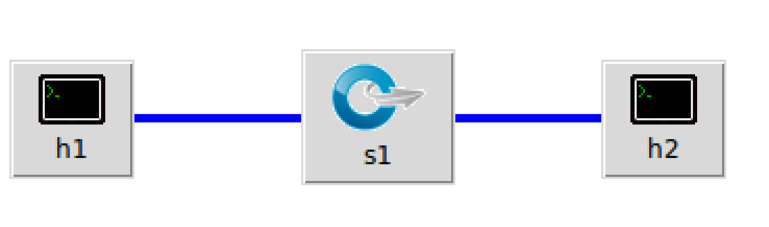
\includegraphics[width=\textwidth]{simple_topo}
	\caption{简单拓扑}
	\label{fig:simpletopo}
\end{figure}
一是简单的两个主机用一个交换机相连,在\ref{fig:simpletopo} 所示,其中h1是QUIC/TCP服务端,h2是QUIC/TCP客户端,S1是交换机。

\begin{figure}
	\centering
	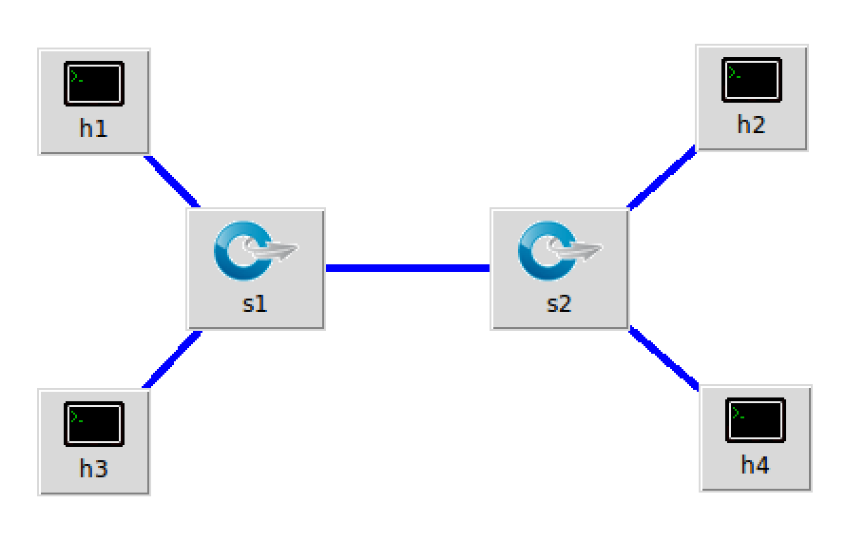
\includegraphics[width=\textwidth]{dumbbell_topo}
	\caption{哑铃型拓扑}
	\label{fig:dumbbelltopo}
\end{figure}
\subsection{流量模式}
二是一个哑铃型拓扑,\ref{fig:dumbbelltopo}所示,其中h1是TCP服务端,h2是TCP客户端,h3是QUIC服务端,h4是QUIC客户端,s1和s2是两个交换机,其中s1和s2之间的链路是瓶颈链路。

使用了两种流量模式:
第一种是由客户端持续发送一定时间的随机生成的字符串。
第二种是由客户端根据泊松流分布进行数据的发送。泊松流

\section{仿真环境}
在这一部分主要讲介绍一下本实验的仿真环境设置。主要包括整个代码运行的环境,以及仿真工具Mininet的简单介绍和接口使用,客户端和服务端的代码逻辑设计。
\subsection{开发环境}
开发环境使用的是由Mac OS X操作系统下的VMware Fusion软件下运行的Ubuntu14.04,64位桌面版的虚拟机。

\subsection{仿真工具Mininet}
Mininet是一个能够添加虚拟主机、交换机、控制器和链路的网络模拟器。Mininet的主机能运行标准的Linux网络软件,更好的是他的交换机能支持更多自定义的路由算法和软件定义的工具。Mininet拥有Python代码的接口,因此非常易于使用,在本章的实验中,将利用Mininet构造不同的网络拓扑,并修改相对应的网络参数,来对QUIC协议和TCP协议进行测试。下面以哑铃型拓扑为例,给出相应的Python代码。

\begin{lstlisting}[language={python},numbers=left]
class XTopo(Topo):
    def build(self, mid_bw, **opts):
        h1 = self.addHost('h1', ip="192.168.0.1/24", mac="cc:cc:cc:cc:cc:01")
        h2 = self.addHost('h2', ip="192.168.0.2/24", mac="cc:cc:cc:cc:cc:02")
        h3 = self.addHost('h3', ip="192.168.0.3/24", mac="cc:cc:cc:cc:cc:03")
        h4 = self.addHost('h4', ip="192.168.0.4/24", mac="cc:cc:cc:cc:cc:04")
        s1 = self.addSwitch('s1')
        s2 = self.addSwitch('s2')
        self.addLink(h1, s1, **opts)
        self.addLink(h2, s2, **opts)
        self.addLink(h3, s1, **opts)
        self.addLink(h4, s2, **opts)
        self.addLink(s1, s2, mid_bw)

    @staticmethod
    def create_net(mid_bw, **opts):
        return Mininet(topo=XTopo(mid_bw, **opts), link=TCLink)
\end{lstlisting}

\subsection{服务端、客户端、仿真程序代码逻辑}
客户端程序实现的功能是根据选择的流量模式,在连接到服务端之后,在一定时间内向服务端发送数据。
服务端程序实现的功能是在每次成功接收到数据之后,统计已经接受到的数据字节数总和并在每次接收到数据的同时输出到终端。仿真程序(即基于Mininet的测试脚本)会定时监视服务端的输出结果,从而来进行数据传输的统计。紧接上一部分哑铃型拓扑的构造,在测试部分对Mininet的接口使用代码如下,其中data1和data2分别都是监控TCP和QUIC协议服务端得到的数据量大小,通过对data1和data2的统计,即可知道两种协议在当前网络状态下的传输吞吐量。
\begin{lstlisting}[language={python},numbers=left]
    while h1.waiting and h3.waiting:
        data1 = h1.monitor(timeoutms=RUN_TIME * 2 * 1000)
        data2 = h3.monitor(timeoutms=RUN_TIME * 2 * 1000)
\end{lstlisting}

\section{仿真结果}
\subsection{仿真结果表格}

\subsection{丢包率的影响}
\subsection{链路带宽的影响}
\subsection{瓶颈电路的影响}
\subsection{不同流量模式的结果}
\section{实际网络环境测试方案}
\subsection{这块的实验:相近网络环境下不同机器之间传输随机字符串所需要的时间}
\section{实际环境测试结果}
\section{本章小结}


